\documentclass[10pt,a4paper]{article}
\usepackage[utf8]{inputenc}
\usepackage[catalan]{babel}
\usepackage{amsmath}
\usepackage{amsfonts}
\usepackage{amssymb}
\usepackage{graphicx}
\usepackage{url}
\author{Martínez Villaronga, Adrià Agustí\\Puigcerver i Pérez, Joan}
\title{Sistema de planificació\\Domini Port}
\begin{document}
\maketitle
\section*{Descripció del problema}
L'objectiu del treball era definir un domini que representara un port
on hi ha diferents blocs apilats en diverses piles a dos molls diferents.
Cada moll pot tindre una sèrie de grues per manipular els blocs i existeix
una cinta per transportar els blocs d'un moll a l'altre. El problema
també especifica que les piles hauran de tindre una alçada màxima
que no es podrà superar en cap cas.\\
El planificador haurà de ser capaç de deixar disponibles a un moll
concret una sèrie de blocs objectiu. Per a que un bloc estiga
disponible a distar dalt de tot d'una pila o, en cas de no estar-ho,
només pot estar a sota d'altres blocs objectiu.
\section*{Dominis}
\subsection*{Versió 1: Domini simplificat}
La primera versió del domini és una simplificació de les especificacions
per tal d'abordar el problema amb més facilitat. S'han eliminat les restriccions
d'alçada de forma que una pila pot creixer indefinidament. Tampoc s'han diferenciat
blocs objectiu de blocs normals, eliminant també el concepte de disponible.\\
Esta primera versió consta de quatre regles: \texttt{pick-from-stack}, \texttt{put-on-stack},
\texttt{pick-from-tape} i \texttt{put-on-tape}.

\subsection*{Versió 2: Introduïnt blocs objectius}
La introducció de blocs objectius va ser el següent pas en la modelització del domini.
Els blocs objectius són un tipus d'objecte diferent dels blocs normals. La modelització
de l'estat disponible o no disponible ha requerit el desdoblament de cada regla
\texttt{pick-from-stack} i \texttt{put-on-stack} en quatre regles diferents,
segons la combinació de bloc normal i bloc objectiu.\\
Segons la forma com s'ha modelat podria donar-se que un bloc objectiu estiga marcat
com a disponible sense estar-ho realment (Figura \ref{fig:fake_disp}), malgrat això
no suposarà un problema ja que quedarà un bloc objectiu no disponible, impedint
que es complisquen els objectius fins que estiguen tots realment disponibles.

\begin{figure}[h]
\centering
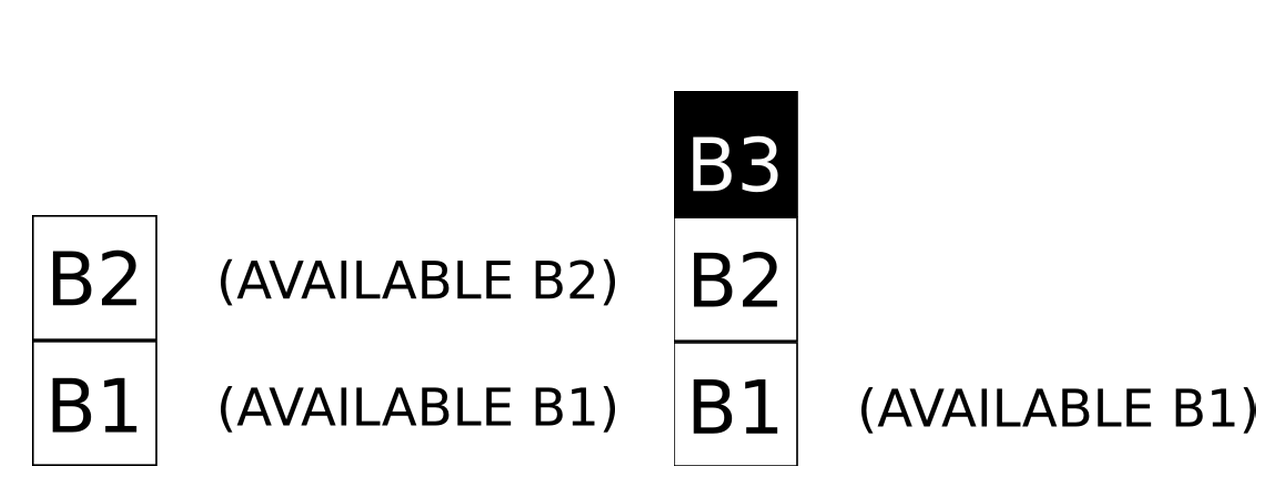
\includegraphics[width=0.6\textwidth]{fake_disp}
\caption{Exemple de fals disponible}
\label{fig:fake_disp}
\end{figure}

\subsection*{Versió 3: Control d'alçada}
La versió 3 representa el domini port complet sense cap extensió, tal
com s'especificava a la definició del domini. Per al control d'alçada 
de les piles s'ha definit un tipus \texttt{HEIGHT} i una sèrie predicats
per indicar quin valor d'alçada és anterior i posterior a un valor donat.

\subsection*{Versió 4: Múltiples cintes}
Una extensió proposada era la d'afegir més de dos molls i per tant més d'una cinta
per poder unir els diferents molls. Aquesta extensió està modelada a la versió 4
del domini. Per fer-ho s'ha definit un tipus cinta i s'han modificat els predicats
i les regles de la cinta per poder indicar a quina cinta fan referència.

\subsection*{Versió 5: Ús de \texttt{fluents} per al control de l'alçada}
Partint de la versió 4 del domini, s'ha fet ús de funcions per modelar el control
de l'alçada de les piles. Aquesta representació del domini elimina alguns tipus 
i predicats així com molts fets de la definició del problema, a més de fer el codi
una mica més llegible. Una particularitat d'aquest domini és que no funciona amb
el planificador \textit{LPG}, donant una violació de segment, mentre que amb
\textit{Metric-FF} no dóna cap problema. No tenim clar el motiu d'aquesta violació
de segment, però possiblement siga degut a que el problema és massa gran.

\subsection*{Versió 6: Domini temporal}
La versió 5 s'havia proposat com un pas intermig per abordar la definició d'un domini temporal
però davant la impossibilitat d'executar-lo en \textit{LPG} vam abordar el domini temporal
a partir de la versió 4. En aquesta versió del domini les accions tenen un cost temporal
associat, tot i que aquest cost és constant a cada acció. Les condicions de les accions poden
haver-se de complir al principi, al final o al llarg de tota l'acció; i els efectes poden
ser efectius al principi o al final de l'acció.

\subsection*{Versió 7: Domini temporal amb \texttt{fluents}}
Aquest domini és una combinació dels dominis de les versions 5 i 6, és a dir, un domini amb funcions duratives
l'alçada de les piles està modelada mitjançant \texttt{fluents}. El problema d'aquest domini és que amb problemes
complexos el planificador es queda penjat al pas \textit{Computing mutex...}. La versió \textbf{7b}, on s'han eliminat
les restriccions d'alçada de les piles, no presenta aquest problema.

\subsection*{Versió 8: Simplificant la codificació del domini}
Aquesta versió no afegeix cap funcionalitat al domini sinó que simplifica la definició
d'aquest combinant les regles \texttt{pick-from-stack-oo} i \texttt{pick-from-stack-ob} en una nova regla \texttt{pick-from-stack-oANY}
i el mateix ocorre amb les regles d'apilar. També s'ha eliminat el tipus \texttt{BOOTOM}. Igual que al domini anterior hi ha un versió
\textbf{8b} sense restriccions d'alçada que no es queda penjada en problemes grans.

\subsection*{Versió 9: Durades dinàmiques}
A partir de la versió 8 s'ha definit aquesta extensió al domini on la durada de les accions és dinàmica en
funció de l'alçada de la pila sobre la qual s'està realitzant l'acció. També s'ha eliminat el predicat \texttt{AT\_STACK} que era redundant.


\section*{Problemes}

\subsection*{Problema 1}
Problema molt senzill per validar la versió 1 del domini. L'objectiu és aconseguir que certs blocs estiguen
apilats un ordre i una posició donades.

\subsection*{Problema 2}
Simplificació del problema proposat (problema 3) sense les restriccions d'alçada màxima per poder provar la versió 2 del domini.

\subsection*{Problema 3}
El problema 3 és el problema proposat a l'enunciat del treball, hi ha diferents versions per provar-lo amb diferents dominis. L'alçada màxima de les piles és 3.

\begin{figure}[h]
\centering
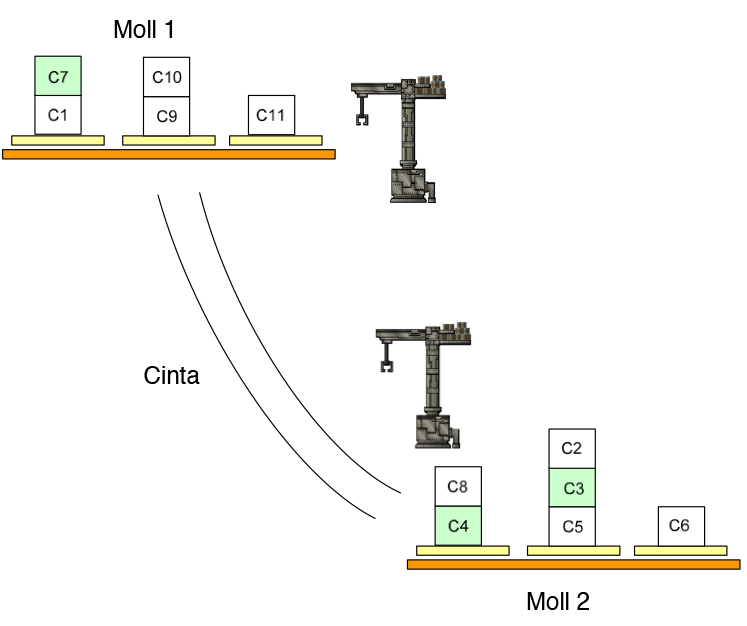
\includegraphics[width=0.6\textwidth]{prob123}
\caption{Disposició inicial dels problemes 1, 2 i 3}
\label{fig:p123}
\end{figure}

\subsection*{Problema 4}
Aquest problema és similar al 3 però més complex, de forma que que la restricció d'alçada màxima (2 en aquest cas) juga un paper
molt important de cara a trobar una solució al poblema. També disposa de diferents versions per als diferents dominis.

\begin{figure}[h]
\centering
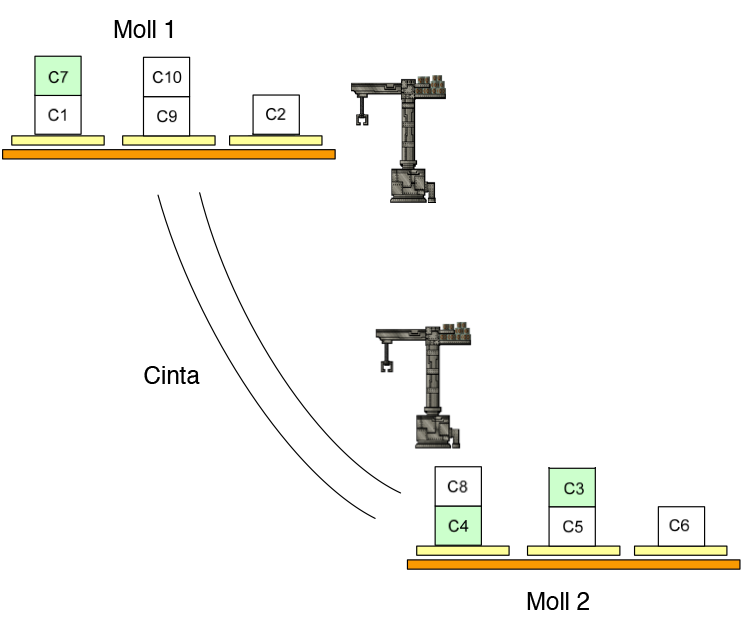
\includegraphics[width=0.6\textwidth]{prob4}
\caption{Disposició inicial del problema 4}
\label{fig:p4}
\end{figure}

\subsection*{Problema 5}
Problema xicotet que força a l'ús de gairebé totes les regles per provar el correcte funcionament d'aquestes.

\begin{figure}[h]
\centering
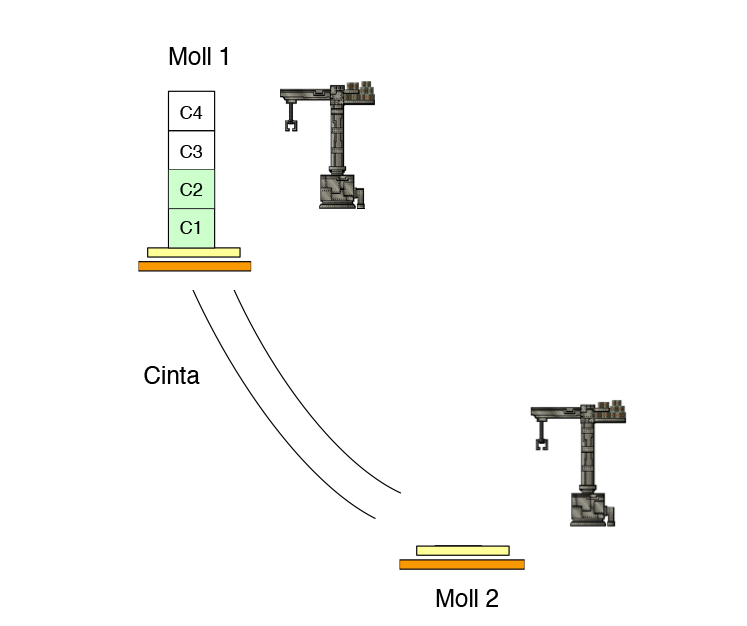
\includegraphics[width=0.6\textwidth]{prob5}
\caption{Disposició inicial del problema 5}
\label{fig:p5}
\end{figure}

\subsection*{Problema simple}
Aquest problema és extremadament senzill consta de dos molls, una pila a cada moll, un bloc normal i un bloc objectiu. Aquest
problema s'ha definit per comprovar el funcionament de les versions 7 i 8 dels dominis que es queden penjades en problemes
més grans.

\begin{figure}[h]
\centering
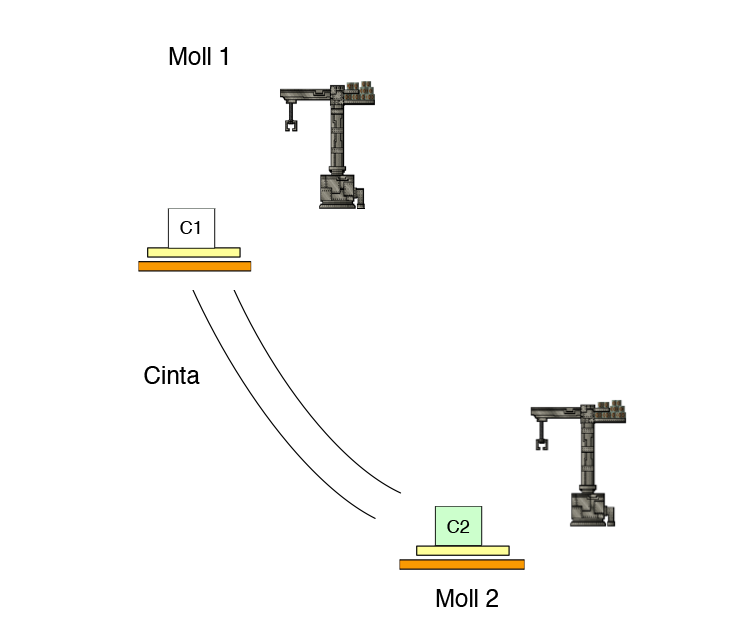
\includegraphics[width=0.6\textwidth]{probS}
\caption{Disposició inicial del problema simple}
\label{fig:pS}
\end{figure}

\section*{Repositori Git}
El projecte està allojat a GitHub a l'adreça \url{https://github.com/jpuigcerver/sirad-harbor}.
Des d'aquesta adreça es pot accedir a tots els dominis i tots els problemes, així com als plans
gereats pels planificadors per als diferents dominis i problemes (carpeta \texttt{plans}).

\end{document}